%+----------------------------------------------------------------------------+
%| SLIDES: Constraint Algebras of multisymplectic Observables (Follow-up talk)
%| Contents:	- 25 minutes (extimated duration ~2 minutes per slide, ~12 slides )
%|
%| Author: Antonio miti
%| Event: 19th International Young Researchers Workshop on Geometry, Dynamics and Field Theory
%| Place: Verona
%| Date: 20/01/25
%+----------------------------------------------------------------------------+


%- HandOut Flag -----------------------------------------------------------------------------------------
	\newif\ifHandout
	%\Handouttrue  %uncomment for the printable version
	%Handling of flags it is not preserved when passing to standalone-subfiles!


%- D0cum3nt ----------------------------------------------------------------------------------------------
\ifHandout
	\documentclass[handout,10pt]{beamer}   
	\setbeameroption{show notes} %print notes   
\else
	\documentclass[10pt]{beamer}
\fi




%- Packages ----------------------------------------------------------------------------------------------
\usepackage{custom-style}
\usepackage{math}









%--Beamer Style-----------------------------------------------------------------------------------------------
\usetheme{toninus}


\usetikzlibrary{backgrounds}
  \tikzset{
    invisible/.style={opacity=0},
    visible on/.style={alt=#1{}{invisible}},
    alt/.code args={<#1>#2#3}{%
      \alt<#1>{\pgfkeysalso{#2}}{\pgfkeysalso{#3}} % \pgfkeysalso doesn't change the path
    },
  }


%- T1tle P4g3 -------------------------------------------------------------------------------------------
\title{ Constraint Algebras \\ of Multisymplectic Observables } 
\subtitle{\href{https://sites.google.com/view/xix-yrw-verona/home?authuser=0}{19th International Young Researchers Workshop on Geometry, Dynamics and Field Theory}}
\author[AMM]{
	\href{https://www.antoniomiti.it/}{Antonio Michele Miti}
	{\small joint work w/ Leonid Ryvkin}
}
\institute[SUR]{
	Sapienza Università di Roma \\
	Rome, Italy 	\\
	\vspace{.5em}
  \begin{tabular}[h]{ccc}
      \href{https://www.mat.uniroma1.it/en}{
\includegraphics[width=6cm]{./Logos/Sur_logo}} & & 
      \href{https://civis3i.univ-amu.fr/en/civis3i-alliance-programme}{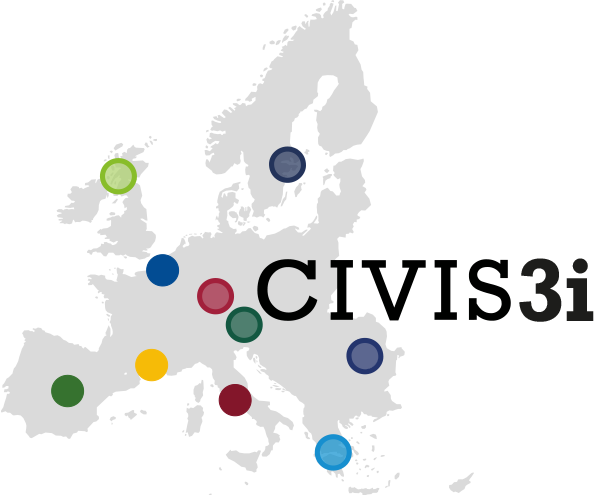
\includegraphics[width=3cm]{Logos/Civis_logo}}
  \end{tabular}    
}
\date[YGMC] % (optional, should be abbreviation of conference name)
{	
	{\vskip 1ex}
	University of Verona, Italy, January 2025
}












%--------------------------------------------------------------------------------------------------
%- D0cum3nt ----------------------------------------------------------------------------------------------------------------------------------
\begin{document}
%------------------------------------------------------------------------------------------------
\begin{frame}  % Alternative: \maketitle outside of frame
	\titlepage
	\ifHandout
		\tikz[overlay,remember picture]
		{
	    	%	\node at ($(current page.west)+(1.5,0)$) [rotate=90] {\Huge\textcolor{gray}{\today}};
	    	\node[        
	    		draw,
	    		shape border rotate=90,
			isosceles triangle,
			isosceles triangle apex angle=90,
			fill=yellow]
	        		at ($(current page.north east)-(1,1)$) [rotate=-45] {\textcolor{red}{Handout version}};
		}
	\fi
\end{frame}
\addtocounter{framenumber}{-1}
\note{
	%\textbf{\underline{OUTLINE}}:
	%\tableofcontents
	\textbf{Abstract:}
	\\
%
This talk explores key algebraic structures in multisymplectic geometry, a generalization of symplectic geometry where higher-degree $k$-forms replace 2-forms. A central theme is the interplay between symmetries (group actions preserving the differential form) and reduction, which constructs a lower-dimensional space inheriting the geometric structure of the original manifold.

The Marsden--Weinstein--Meyer theorem in symplectic geometry connects this reduction process to regular-level sets of momentum maps, with extensions to singular cases by Śniatycki and Weinstein. Marvin Dippel, Chiara Esposito, and Stephan Waldmann (\href{https://arxiv.org/abs/2310.05613}{\texttt{arXiv:2310.05613}}) developed a framework for constraint algebras of observables in the context of coisotropic reduction in Poisson geometry. 

Our research builds on previous work by adapting and implementing algebraic reduction schemes within multisymplectic geometry, providing a higher-dimensional perspective on the relationship between symmetries and reduction.

This talk reviews higher versions of observable algebras and moment maps in multisymplectic geometry and examines how regular and singular reduction schemes extend to this framework. The presentation is based on ongoing joint work with Leonid Ryvkin.


}
%--------------------------------------------------------------------------------------------------




%------------------------------------------------------------------------------------------------
\begin{frame}[fragile]{Keywords}
\tikzstyle{every picture}+=[remember picture]
	\begin{columns}
    	\begin{column}{.45\textwidth}
    		\onslide<4->{
			\tikz[baseline]{
		            \node[draw=orange!40,anchor=base,text width=5cm] (s1)
		            {Algebraic structure encoding informations necessary for defining coisotropic reduction in Poisson geometry.};
			}
		}
	\end{column}
    	\begin{column}{.45\textwidth}
    		\onslide<5->{
			 \tikz[baseline]{
		            \node[draw=blue!40,anchor=base, text width=5cm] (s2)
		            {Mathematical formalization of classical measurable quantities.};
			}
		}
	\end{column}
	\end{columns}

	\vfill

	\begin{center}
		\large
		 \tikz[baseline]{
		            \node[fill=orange!20,anchor=base] (t1)
		            {Constraint Algebra};
			}
		\\
		of 
		\\
		 \tikz[baseline]{
	            \node[fill=green!20,anchor=base] (t3)
	            {Multi};
		}
		\kern-3pt - \kern-3pt
		 \tikz[baseline]{
	            \node[fill=red!20,anchor=base] (t4)
	            {Symplectic};
		}		
		  \tikz[baseline]{
		            \node[fill=blue!20,anchor=base] (t2)
		            {Observables};
		        } 

	\end{center}

	\vfill

	\begin{columns}
    	\begin{column}{.45\textwidth}
    		\onslide<3->{
	 		 \tikz[baseline]{
	            \node[draw=green!40,anchor=base,text width=5cm] (s3)
	            {A certain higher version \\(involving differential forms in degree $\geq 2$)};
	         }
		}		   	
		\end{column}
    	\begin{column}{.45\textwidth}
    		\onslide<2->{
				\tikz[baseline]{
	            \node[draw=red!40,anchor=base,text width=5cm] (s4)
	            {Closed $2$-form on a smooth manifold, providing a geometric framework for classical mechanics};
	           }	
			}
		\end{column}
	\end{columns}

	\begin{tikzpicture}[overlay]
        \path[->,draw=orange!40]<4-> (s1) edge [bend right] (t1);
        \path[->,draw=blue!40]<5-> (s2) edge [bend left] (t2);
        \path[->,draw=green!40]<3-> (s3) edge [bend left] (t3);
        \path[->,draw=red!40]<2-> (s4) edge [bend left] (t4);
	\end{tikzpicture}

	\vfill
	\onslide<1->{
	\begin{block}{Based on:}
%		 \emph{ \small
%			 Blacker, M, Ryvkin;
%			\textbf{Reduction of $L_\infty$-algebra of observables on multisymplectic manifolds}; 
%			\href{https://arxiv.org/abs/2206.03137}{arXiv:2206.03137}.
%		}
%		\\
		 \emph{ \small
			 M. , Ryvkin;
			\textbf{Constraint algebras of multisyplectic observables}; 
			\href{https://www.antoniomiti.it/teaching/Obs-Constraint-2024/}{In preparation}.
		}		
	\end{block}
	}

\end{frame}
\note[itemize]{
	\item Provide a vague idea of the words that make up the title.
	\item \cite{Dippell2023}
	\item Conventions:
	\\- $M$ and $G$ are connected,
	\\- actions $\theta:G \curvearrowright M$ are always smooth
	\\- $\xi,\eta\in\g$,
	\\- for $\mu\in\Omega^*(M,\g^*)$ and $\xi\in\g$, write
			\[
				\mu_\xi := \langle\mu,\xi\rangle \;{\color{black!50}\in\Omega^*(M)}
			\]
			for the ``$\xi$th component'' of $\mu$.
}
%------------------------------------------------------------------------------------------------

\end{document}

%------------------------------------------------------------------------------------------------
\section{Symplectic Reduction}
\checkpoint	
%------------------------------------------------------------------------------------------------


%------------------------------------------------------------------------------------------------
\section{Multisymplectic Geometry}
\checkpoint	
%------------------------------------------------------------------------------------------------




%------------------------------------------------------------------------------------------------
\section{Multisymplectic observables reduction}
\checkpoint	
%------------------------------------------------------------------------------------------------








%------------------------------------------------------------------------------------------------
% APPENDIX
%------------------------------------------------------------------------------------------------
\appendix
%------------------------------------------------------------------------------------------------

%	\includestandalone{msconstraints-appendix}

	\includestandalone{msconstraints-aknowledgements}
%------------------------------------------------------------------------------------------------










%------------------------------------------------------------------------------------------------
\end{document}

